%%%%%%%%%%%%%%%%%%%%%%%%%%%%%%%%%%%%%%%%%%%%%%%%%%%
%% LaTeX book template                           %%
%% Author:  Amber Jain (http://amberj.devio.us/) %%
%% License: ISC license                          %%
%%%%%%%%%%%%%%%%%%%%%%%%%%%%%%%%%%%%%%%%%%%%%%%%%%%

\documentclass[a4paper,11pt,oneside]{book}
\usepackage{../../modulestyle}

%%%%%%%%%%%%%%%%%%%%%%%%%%%%%%%%%%%%%%%%%%%%%%%%%%%%%%%%%
% Source: http://en.wikibooks.org/wiki/LaTeX/Hyperlinks %
%%%%%%%%%%%%%%%%%%%%%%%%%%%%%%%%%%%%%%%%%%%%%%%%%%%%%%%%%

%%%%%%%%%%%%%%%%%%%%%%%%%%%%%%%%%%%%%%%%%%%%%%%%%%%%%%%%%%%%%%%%%%%%%%%%%%%%%%%%
% 'dedication' environment: To add a dedication paragraph at the start of book %
% Source: http://www.tug.org/pipermail/texhax/2010-June/015184.html            %
%%%%%%%%%%%%%%%%%%%%%%%%%%%%%%%%%%%%%%%%%%%%%%%%%%%%%%%%%%%%%%%%%%%%%%%%%%%%%%%%
\newenvironment{dedication}
{
   \cleardoublepage
   \thispagestyle{empty}
   \vspace*{\stretch{1}}
   \hfill\begin{minipage}[t]{0.66\textwidth}
   \raggedright
}
{
   \end{minipage}
   \vspace*{\stretch{3}}
   \clearpage
}

%%%%%%%%%%%%%%%%%%%%%%%%%%%%%%%%%%%%%%%%%%%%%%%%
% Chapter quote at the start of chapter        %
% Source: http://tex.stackexchange.com/a/53380 %
%%%%%%%%%%%%%%%%%%%%%%%%%%%%%%%%%%%%%%%%%%%%%%%%
\makeatletter
\renewcommand{\@chapapp}{}% Not necessary...
\newenvironment{chapquote}[2][2em]
  {\setlength{\@tempdima}{#1}%
   \def\chapquote@author{#2}%
   \parshape 1 \@tempdima \dimexpr\textwidth-2\@tempdima\relax%
   \itshape}
  {\par\normalfont\hfill--\ \chapquote@author\hspace*{\@tempdima}\par\bigskip}
\makeatother

%%%%%%%%%%%%%%%%%%%%%%%%%%%%%%%%%%%%%%%%%%%%%%%%%%%
% First page of book which contains 'stuff' like: %
%  - Book title, subtitle                         %
%  - Book author name                             %
%%%%%%%%%%%%%%%%%%%%%%%%%%%%%%%%%%%%%%%%%%%%%%%%%%%

\newcommand{\CourseTitle}{Object-Oriented Programming}
\newcommand{\ChapterNumber}{1}
\newcommand{\ChapterTitle}{Introduction to Object-Oriented Programming}
\newcommand{\CodingNumber}{1.3.11}
\newcommand{\CodingTitle}{Hello, World!}
\newcommand{\SubmissionDeadline}{October 4, 2024}
\newcommand{\SubmissionDeadlineText}{on or before \SubmissionDeadline}
\newcommand{\SubmissionTemplateURL}{https://docs.google.com/document/d/1sctvVLgpPSVnXN82k6LsOPSPApKp2rV0/edit?usp=drive_link&ouid=112709378145681657270&rtpof=true&sd=true}

\newcommand{\BookTitle}{Coding Exercise: \CodingNumber - \CodingTitle}
\newcommand{\BookTitleFootnote}{A coding exercise for
Chapter \ChapterNumber of the Study Guide on the course \CourseTitle.}

\newcommand{\BookSubtitle}{Chapter \ChapterNumber: \ChapterTitle}
\newcommand{\BookSubtitleFootnote}{This chapter introduces the basic concepts
of Object-Oriented Programming and Java programming language.}

\newcommand{\BookAuthorFirstName}{Jarrian Vince}
\newcommand{\BookAuthorLastName}{Gojar}
\newcommand{\BookAuthorName}{Jarrian Vince G. Gojar}
\newcommand{\BookAuthorURL}{https://github.com/godkingjay}

\newcommand{\GoogleDriveURLBSCSTwoOne}{https://drive.google.com/drive/folders/1c56xFCJgFh6FWQQ4iZ-UuKKcWioF8pgs?usp=sharing}
\newcommand{\GoogleDriveURLBSCSTwoTwo}{https://drive.google.com/drive/folders/1jANc3o6atOYbHyoJZ6b-j-nDlTknEiu-?usp=sharing}

\newcommand{\FolderFormat}{Group Number - LastName1\_FirstName1, LastName2\_FirstName2}
\newcommand{\FolderFormatExample}{Group 1 - Doe\_John, Smith\_Jane}

% Book's title and subtitle
\title{\Huge \textbf{\BookTitle}  \footnote{\BookTitleFootnote} \\
\huge \BookSubtitle \footnote{\BookSubtitleFootnote}}

% Author
\author{\textsc{\BookAuthorName}\thanks{\url{\BookAuthorURL}}}

\begin{document}

\frontmatter
\maketitle

%%%%%%%%%%%%%%%%%%%%%%%%%%%%%%%%%%%%%%%%%%%%%%%%%%%%%%%%%%%%%%%
% Add a dedication paragraph to dedicate your book to someone %
%%%%%%%%%%%%%%%%%%%%%%%%%%%%%%%%%%%%%%%%%%%%%%%%%%%%%%%%%%%%%%%
\begin{dedication}
Sorsogon State University - Bulan Campus
\end{dedication}

%%%%%%%%%%%%%%%%%%%%%%%%%%%%%%%%%%%%%%%%%%%%%%%%%%%%%%%%%%%%%%%%%%%%%%%%
% Auto-generated table of contents, list of figures and list of tables %
%%%%%%%%%%%%%%%%%%%%%%%%%%%%%%%%%%%%%%%%%%%%%%%%%%%%%%%%%%%%%%%%%%%%%%%%

\mainmatter

%%%%%%%%%%%
% Preface %
%%%%%%%%%%%
\section*{Coding Exercises}

Instructions: Write a program that solves the following problems.
Submit your code to the Google Drive folder provided by the instructor.

% Red Large Text
\textcolor{red}{\Large{Note 1: You have to answer 2 out of the 4 exercises.}}

% Answer 1 and one of the remaining exercises
\textcolor{red}{\Large{Note 2: You have to answer Exercise 1 and one of the
remaining exercises. (e.g., Exercise 1 and Exercise 2, Exercise 1 and Exercise
3, etc.)}}

\begin{enumerate}
  \item Write a program that prints "Hello, World!" to the console.
  \item Write a program that calculates the area of a triangle given the base
  and height and prints the result to the console.
  \begin{align*}
    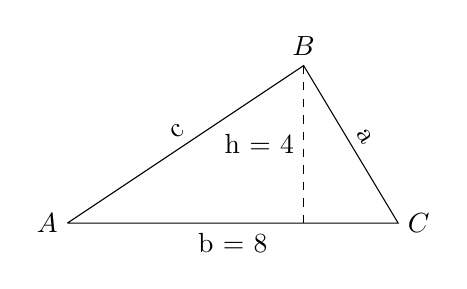
\begin{tikzpicture}[scale=1]
      \coordinate [label=left:$A$] (A) at (-2cm,-1.cm);
      \coordinate [label=right:$C$] (C) at (2.2cm,-1.0cm);
      \coordinate [label=above:$B$] (B) at (1cm,1.0cm);
      \draw (A) -- node[sloped,above] {c} (B) -- node[sloped,above,] {a} (C) -- node[below] {b = 8} (A);
      \draw[dashed] (B) -- node[left] {h = 4} (A-|B);
    \end{tikzpicture}
  \end{align*}
  \begin{align}
    b &= 8 \text{, the base of the triangle} \\
    h &= 4 \text{, the height of the triangle} \\
    A &= \frac{b \cdot h}{2} \text{, formula for the area of a triangle}
  \end{align}
  \item Write a program that calculates the area of a rectangle given the
  length and width and prints the result to the console.
  \begin{align*}
    \begin{tikzpicture}[scale=1]
      \coordinate [label=left:$A$] (A) at (-2cm,1cm);
      \coordinate [label=right:$B$] (B) at (2cm,1cm);
      \coordinate [label=right:$C$] (C) at (2cm,-1cm);
      \coordinate [label=left:$D$] (D) at (-2cm,-1cm);
      \draw (A) -- node[above] {w = 4} (B) -- node[right] {l = 2} (C) -- (D) -- (A);
    \end{tikzpicture}
  \end{align*}
  \begin{align}
    l &= 2 \text{, the length of the rectangle} \\
    w &= 4 \text{, the width of the rectangle} \\
    A &= l \cdot w \text{, formula for the area of a rectangle}
  \end{align}
  \item Write a program that calculates the area of a circle given the radius
    and prints the result to the console.
  \begin{align*}
    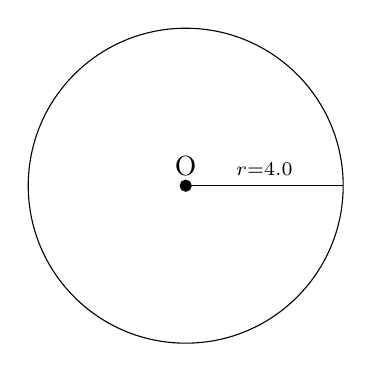
\begin{tikzpicture}[scale=1]
      \draw (2,2) circle (2cm);
      \draw[fill=black](2,2) circle (2 pt) node [above] {O};
      \draw[](2,2) -- (4,2) node [midway,above] {$\scriptstyle r = 4.0$};
    \end{tikzpicture}
  \end{align*}
  \begin{align}
    r &= 4.0 \text{, the radius of the circle} \\
    \pi &= 3.141592653589793 \text{, the mathematical constant pi} \\
    A &= \pi \cdot r^2 \text{, formula for the area of a circle}
  \end{align}
\end{enumerate}

\section*{Submission of Coding Exercises}

Instructions:
\begin{enumerate}
  \item Go to the Google Drive folder provided by the instructor: \\
  \begin{quote}
    \textbf{For BSCS 2-1:} \\
    \url{\GoogleDriveURLBSCSTwoOne} \\ \\
    \textbf{For BSCS 2-2:} \\
    \url{\GoogleDriveURLBSCSTwoTwo}
  \end{quote}
  \item Inside the folder, create another folder for your group
  with the following format:
    \begin{quote}
      \textbf{\FolderFormat} \\
      Example: \textbf{\FolderFormatExample}
    \end{quote}
  \item Inside the sub-folder, create another folder with the name:
    \begin{quote}
        \textbf{Chapter \ChapterNumber - Coding Exercise \CodingNumber - \CodingTitle}
    \end{quote}
  \item Inside the folder, upload the file of your submission.
    \begin{quote}
        Fill in the template provided in the following link and upload
        it inside the folder: \\
        \url{\SubmissionTemplateURL}
    \end{quote}
  \item The activity must be submitted \textbf{\SubmissionDeadlineText}.
  \item Late submissions will not be accepted.
\end{enumerate}

\end{document}